\documentclass[14pt]{extbook}
\usepackage{multicol, enumerate, enumitem, hyperref, color, soul, setspace, parskip, fancyhdr} %General Packages
\usepackage{amssymb, amsthm, amsmath, bbm, latexsym, units, mathtools} %Math Packages
\everymath{\displaystyle} %All math in Display Style
% Packages with additional options
\usepackage[headsep=0.5cm,headheight=12pt, left=1 in,right= 1 in,top= 1 in,bottom= 1 in]{geometry}
\usepackage[usenames,dvipsnames]{xcolor}
\usepackage{dashrule}  % Package to use the command below to create lines between items
\newcommand{\litem}[1]{\item#1\hspace*{-1cm}\rule{\textwidth}{0.4pt}}
\pagestyle{fancy}
\lhead{Progress Quiz 8}
\chead{}
\rhead{Version C}
\lfoot{4553-3922}
\cfoot{}
\rfoot{Fall 2020}
\begin{document}

\begin{enumerate}
\litem{
Describe the end behavior of the polynomial below.\[ f(x) = 6(x + 4)^{3}(x - 4)^{4}(x + 9)^{3}(x - 9)^{3} \]\begin{enumerate}[label=\Alph*.]
\begin{multicols}{2}\item 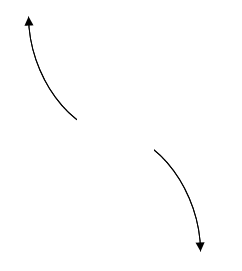
\includegraphics[width = 0.3\textwidth]{../Figures/polyEndBehaviorAC.png}\item 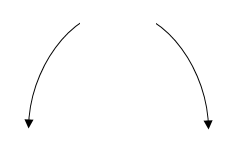
\includegraphics[width = 0.3\textwidth]{../Figures/polyEndBehaviorBC.png}\item 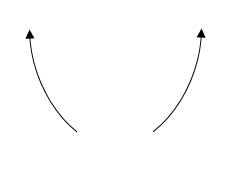
\includegraphics[width = 0.3\textwidth]{../Figures/polyEndBehaviorCC.png}\item 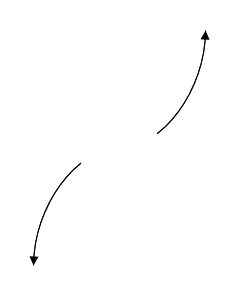
\includegraphics[width = 0.3\textwidth]{../Figures/polyEndBehaviorDC.png}\end{multicols}\item None of the above.
\end{enumerate} }
\litem{
Construct the lowest-degree polynomial given the zeros below. Then, choose the intervals that contain the coefficients of the polynomial in the form $ax^3+bx^2+cx+d$.\[ \frac{-3}{2}, \frac{1}{5}, \text{ and } 6 \]\begin{enumerate}[label=\Alph*.]
\item \( a \in [6, 11], b \in [47, 50], c \in [-83, -76], \text{ and } d \in [-21, -15] \)
\item \( a \in [6, 11], b \in [-55, -41], c \in [-83, -76], \text{ and } d \in [-21, -15] \)
\item \( a \in [6, 11], b \in [-55, -41], c \in [-83, -76], \text{ and } d \in [16, 25] \)
\item \( a \in [6, 11], b \in [-74, -70], c \in [75, 80], \text{ and } d \in [16, 25] \)
\item \( a \in [6, 11], b \in [-80, -75], c \in [101, 114], \text{ and } d \in [-21, -15] \)

\end{enumerate} }
\litem{
Describe the zero behavior of the zero $x = -4$ of the polynomial below.\[ f(x) = 6(x - 4)^{9}(x + 4)^{12}(x + 8)^{3}(x - 8)^{5} \]\begin{enumerate}[label=\Alph*.]
\begin{multicols}{2}\item 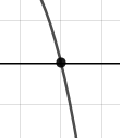
\includegraphics[width = 0.3\textwidth]{../Figures/polyZeroBehaviorCopyAC.png}\item 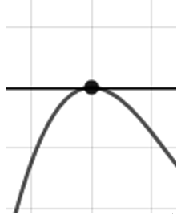
\includegraphics[width = 0.3\textwidth]{../Figures/polyZeroBehaviorCopyBC.png}\item 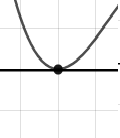
\includegraphics[width = 0.3\textwidth]{../Figures/polyZeroBehaviorCopyCC.png}\item 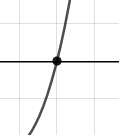
\includegraphics[width = 0.3\textwidth]{../Figures/polyZeroBehaviorCopyDC.png}\end{multicols}\item None of the above.
\end{enumerate} }
\litem{
Construct the lowest-degree polynomial given the zeros below. Then, choose the intervals that contain the coefficients of the polynomial in the form $x^3+bx^2+cx+d$.\[ 5 - 2 i \text{ and } 3 \]\begin{enumerate}[label=\Alph*.]
\item \( b \in [-16, -12], c \in [59, 62], \text{ and } d \in [-89, -75] \)
\item \( b \in [-3, 6], c \in [-13, -5], \text{ and } d \in [14, 20] \)
\item \( b \in [-3, 6], c \in [-4, 0], \text{ and } d \in [-9, 1] \)
\item \( b \in [10, 20], c \in [59, 62], \text{ and } d \in [84, 92] \)
\item \( \text{None of the above.} \)

\end{enumerate} }
\litem{
Which of the following equations \textit{could} be of the graph presented below?
\begin{center}
    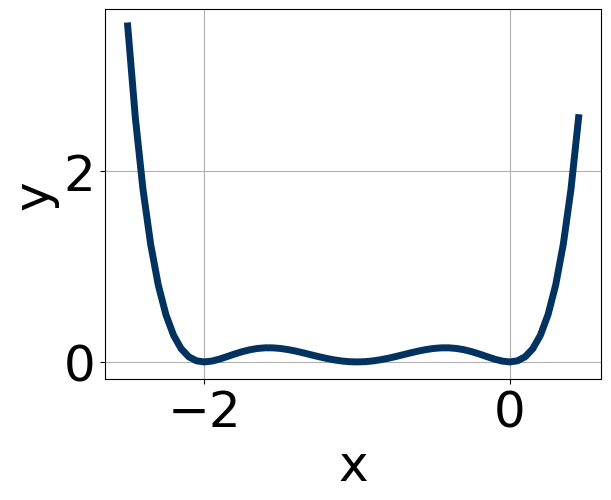
\includegraphics[width=0.5\textwidth]{../Figures/polyGraphToFunctionCopyC.png}
\end{center}
\begin{enumerate}[label=\Alph*.]
\item \( 10x^{4} (x - 1)^{11} (x - 2)^{5} \)
\item \( 10x^{4} (x - 1)^{8} (x - 2)^{9} \)
\item \( -6x^{10} (x - 1)^{6} (x - 2)^{6} \)
\item \( -16x^{6} (x - 1)^{10} (x - 2)^{7} \)
\item \( 10x^{10} (x - 1)^{7} (x - 2)^{4} \)

\end{enumerate} }
\litem{
Describe the zero behavior of the zero $x = 5$ of the polynomial below.\[ f(x) = 6(x - 5)^{8}(x + 5)^{9}(x - 9)^{2}(x + 9)^{6} \]\begin{enumerate}[label=\Alph*.]
\begin{multicols}{2}\item 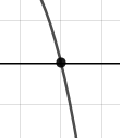
\includegraphics[width = 0.3\textwidth]{../Figures/polyZeroBehaviorAC.png}\item 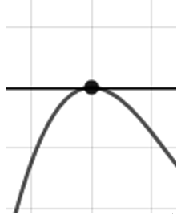
\includegraphics[width = 0.3\textwidth]{../Figures/polyZeroBehaviorBC.png}\item 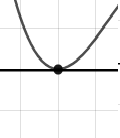
\includegraphics[width = 0.3\textwidth]{../Figures/polyZeroBehaviorCC.png}\item 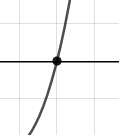
\includegraphics[width = 0.3\textwidth]{../Figures/polyZeroBehaviorDC.png}\end{multicols}\item None of the above.
\end{enumerate} }
\litem{
Describe the end behavior of the polynomial below.\[ f(x) = -9(x - 9)^{3}(x + 9)^{4}(x - 8)^{5}(x + 8)^{6} \]\begin{enumerate}[label=\Alph*.]
\begin{multicols}{2}\item 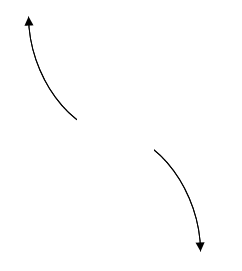
\includegraphics[width = 0.3\textwidth]{../Figures/polyEndBehaviorCopyAC.png}\item 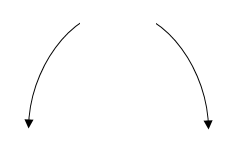
\includegraphics[width = 0.3\textwidth]{../Figures/polyEndBehaviorCopyBC.png}\item 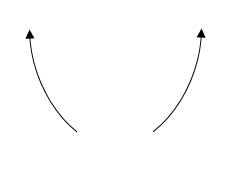
\includegraphics[width = 0.3\textwidth]{../Figures/polyEndBehaviorCopyCC.png}\item 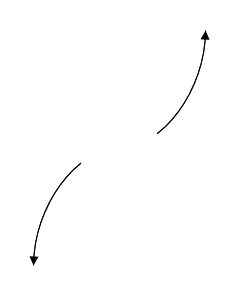
\includegraphics[width = 0.3\textwidth]{../Figures/polyEndBehaviorCopyDC.png}\end{multicols}\item None of the above.
\end{enumerate} }
\litem{
Construct the lowest-degree polynomial given the zeros below. Then, choose the intervals that contain the coefficients of the polynomial in the form $x^3+bx^2+cx+d$.\[ -2 - 4 i \text{ and } -4 \]\begin{enumerate}[label=\Alph*.]
\item \( b \in [7, 12], c \in [33.6, 38.7], \text{ and } d \in [78, 88] \)
\item \( b \in [-8, -3], c \in [33.6, 38.7], \text{ and } d \in [-82, -75] \)
\item \( b \in [-2, 6], c \in [4.5, 7.9], \text{ and } d \in [3, 9] \)
\item \( b \in [-2, 6], c \in [6.8, 9.4], \text{ and } d \in [12, 24] \)
\item \( \text{None of the above.} \)

\end{enumerate} }
\litem{
Construct the lowest-degree polynomial given the zeros below. Then, choose the intervals that contain the coefficients of the polynomial in the form $ax^3+bx^2+cx+d$.\[ \frac{7}{5}, \frac{-4}{5}, \text{ and } \frac{1}{2} \]\begin{enumerate}[label=\Alph*.]
\item \( a \in [50, 51], b \in [-63, -50], c \in [-43, -33], \text{ and } d \in [-32, -26] \)
\item \( a \in [50, 51], b \in [51, 56], c \in [-43, -33], \text{ and } d \in [-32, -26] \)
\item \( a \in [50, 51], b \in [80, 86], c \in [-2, 3], \text{ and } d \in [-32, -26] \)
\item \( a \in [50, 51], b \in [-63, -50], c \in [-43, -33], \text{ and } d \in [24, 36] \)
\item \( a \in [50, 51], b \in [4, 8], c \in [-73, -67], \text{ and } d \in [24, 36] \)

\end{enumerate} }
\litem{
Which of the following equations \textit{could} be of the graph presented below?
\begin{center}
    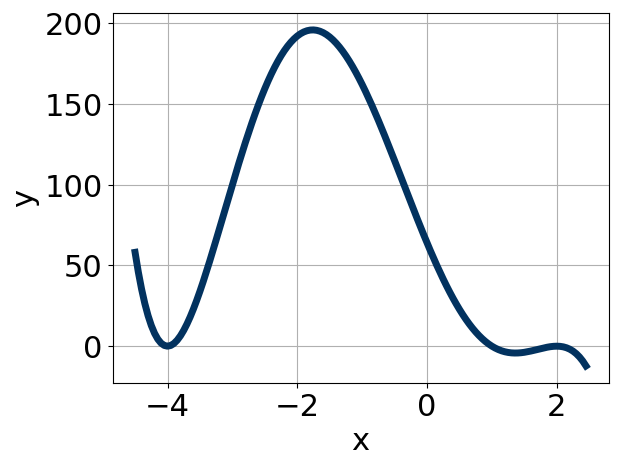
\includegraphics[width=0.5\textwidth]{../Figures/polyGraphToFunctionC.png}
\end{center}
\begin{enumerate}[label=\Alph*.]
\item \( 15x^{7} (x - 1)^{11} (x - 2)^{11} \)
\item \( -13x^{7} (x - 1)^{9} (x - 2)^{7} \)
\item \( 19x^{7} (x - 1)^{8} (x - 2)^{6} \)
\item \( -15x^{5} (x - 1)^{8} (x - 2)^{7} \)
\item \( 7x^{11} (x - 1)^{6} (x - 2)^{9} \)

\end{enumerate} }
\end{enumerate}

\end{document}